\subsection{B1 - Generation of smooth trajectories with polynomial splines}
In this task, we should generate a trajectory that starts at a point in time $t_{start}$ in configuration $q_a$ passes after 2.5s the via configuration $q_b$(referred to as $t_{via}$ in the following) on its way to the final configuration $q_c$ which it reaches at 5s (referred to as $t_{end}$ in the following ). We therefore need to compute for each joint two trajectory splines. One that connects the start to the via (in 2.5s) and one which connects the via to the desired end point. The basic formula was shown in the tutorial of the Robotics course and while the structure of Equation \ref{eq:splineOne} and \ref{eq:splineTwo} seems to be similar the $a_{ij}$ and the time offset is different. 


\begin{equation}
    q(t) = a_{1,1} + a_{1,2} \cdot (t- t_{start}) + a_{1,3} \cdot (t-t_{start})^2 + a_{1,4}\cdot (t-t_{start})^3
    \label{eq:splineOne}
\end{equation}
for $ t_{start} \leq t \leq t_{via}$
\begin{equation}
   q(t) = a_{2,1} + a_{2,2} \cdot (t- t_{via}) + a_{2,3} \cdot (t-t_{via})^2 + a_{2,4}\cdot (t-t_{via})^3
   \label{eq:splineTwo}
\end{equation}

for $ t_{via} \leq t \leq t_f$.

The general formula for the $a_{i,j}$'s was derived in the tutorial of this Robotics course and can be specified for our case as follows. 


\begin{equation}
a_{1,1}=q_a
\end{equation}

\begin{equation}
a_{1,2}=\dot{q_a}
\end{equation}

\begin{equation}
a_{1,3}=\frac{3}{(t_{via}-t_{start})^2}\cdot(q_b-q_a)- \frac{2}{t_{via}-t_{start}}\cdot \dot{q_a}- \frac{1}{t_{via}-t_{start}} \cdot \dot{q_b}
\end{equation}

\begin{equation}
a_{1,4}=-\frac{2}{(t_{via}-t_{start})^3}\cdot(q_b-q_a)+ \frac{1}{(t_{via}-t_{start})^2}\cdot(\dot{q_a}+\dot{q_b})
\end{equation}

\begin{equation}
a_{2,1}=q_b
\end{equation}

\begin{equation}
a_{2,2}=\dot{q_b}
\end{equation}

\begin{equation}
a_{2,3}=\frac{3}{(t_{end}-t_{via})^2}\cdot(q_c-q_b)- \frac{2}{t_{end}-t_{via}}\cdot \dot{q_b}- \frac{1}{t_{end}-t_{via}} \cdot \dot{q_c}
\end{equation}

\begin{equation}
a_{2,4}=-\frac{2}{(t_{end}-t_{via})^3}\cdot(q_c-q_b)+ \frac{1}{(t_{end}-t_{via})^2}\cdot(\dot{q_b}+\dot{q_c})
\end{equation}

As the different joints have different trajectories it is advisable to deduce the spline polynomials for them separately. Starting with $q_1$, we have to think about conditions that allow us to solve the equation of all $a_{ij}$. First of all, to implement a smooth spline trajectory we demand the start and end velocity $\dot{q_a}$ and  $\dot{q_c}$ to be zero. 
In order to, know the via velocity we have to follow the heuristic approach presented to us in the tutorial of this robotics course. When looking at $q_{a1}$= 0, $q_{b1}$= $-\frac{\pi}{4}$ and $q_{c1}$=$-\frac{\pi}{2}$, we can see that that there is no sign change. Therefore we know that the velocity of the via should be the mean velocity that is taken to the via from the start and from the via to the end. As we have a change in angle of -$\frac{\pi}{4}$ in 2.5s in both segments $\dot{q_b}$ can be calculated as: 

\begin{equation}
    \dot{q_b}=\frac{1}{2}\cdot(-\frac{\pi}{4\cdot 2.5s} - \frac{\pi}{4\cdot 2.5s}) = -\frac{\pi}{10}
\end{equation}

Now that enough conditions are established the $a_{ij}$'s can be calculated for the trajectory of angle $q_1$.

\begin{equation}
a_{1,1}=q_a = 0
\end{equation}

\begin{equation}
a_{1,2}=\dot{q_a} = 0
\end{equation}

\begin{equation}
a_{1,3}=\frac{3\cdot(q_b-q_a)}{(t_{via}-t_{start})^2}- \frac{\dot{q_b}}{t_{via}-t_{start}}   = -\frac{2\pi}{25}
\end{equation}

\begin{equation}
a_{1,4}=-\frac{2\cdot(q_b-q_a)}{(t_{via}-t_{start})^3}+ \frac{\dot{q_b}}{(t_{via}-t_{start})^2} \approx 0.05
\end{equation}

\begin{equation}
a_{2,1}=q_b = -\frac{\pi}{4}
\end{equation}

\begin{equation}
a_{2,2}=\dot{q_b} = -\frac{\pi}{10}
\end{equation}

\begin{equation}
a_{2,3}=\frac{3\cdot(q_c-q_b)}{(t_{end}-t_{via})^2}- \frac{2\cdot \dot{q_b}}{t_{end}-t_{via}} = -\frac{\pi}{25}
\end{equation}

\begin{equation}
a_{2,4}=-\frac{2\cdot(q_c-q_b)}{(t_{end}-t_{via})^3}+ \frac{\dot{q_b}}{(t_{end}-t_{via})^2} \approx 0.05
\end{equation}

When inserting the calculated $a_{ij}$'s in the Equation \ref{eq:splineOne} and \ref{eq:splineTwo} the following trajectory spline was determined
for angle $q_1$. 

\begin{equation}
    q_1(t) \approx -\frac{2\pi}{25}  (t-t_{start})^2  + 0.05(t-t_{start})^3
\end{equation}

for the time interval $ t_{start} \leq t \leq t_{via}$ and 

for $ t_{start} \leq t \leq t_{via}$
\begin{equation}
   q_1(t) \approx -\frac{\pi}{4} - \frac{\pi}{10}  (t- t_{via}) -\frac{\pi}{25}  (t-t_{via})^2 + 0.05 (t-t_{via})^3
   \label{eq:splineTwooo}
\end{equation}

for the time interval $ t_{via} \leq t \leq t_{end}$. 

\newline
In contrast to $q_1$ the trajectory of $q_2$ starts at $q_a$=0, passes the via point at $q_b=\frac{\pi}{2}$ and goes back down to $q_c=\frac{\pi}{4}$. As $q_2$ encounters a sign change of the velocity the via velocity $\dot{q_{b2}}$ is zero. The starting and end velocity $\dot{q_{a2}}$ and $\dot{q_{c2}}$ is again assumed to be zero for a smooth trajectory. 
With this conditions $a_{ij}$ can be calculated for trajectory $q_2$

\begin{equation}
a_{1,1}=q_a = 0
\end{equation}

\begin{equation}
a_{1,2}=\dot{q_a} = 0
\end{equation}

\begin{equation}
a_{1,3}=\frac{3\cdot(q_b-q_a)}{(t_{via}-t_{start})^2} = \frac{6\pi}{25}
\end{equation}

\begin{equation}
a_{1,4}=-\frac{2\cdot(q_b-q_a)}{(t_{via}-t_{start})^3} \approx -0.20
\end{equation}

\begin{equation}
a_{2,1}=q_b = \frac{\pi}{2}
\end{equation}

\begin{equation}
a_{2,2}=\dot{q_b} = 0
\end{equation}

\begin{equation}
a_{2,3}=\frac{3\cdot(q_c-q_b)}{(t_{end}-t_{via})^2} = -\frac{3\pi}{25}
\end{equation}

\begin{equation}
a_{2,4}=-\frac{2\cdot(q_c-q_b)}{(t_{end}-t_{via})^3} \approx 0.10
\end{equation}
\newpage
When inserting the calculated $a_{ij}$'s in the Equation \ref{eq:splineOne} and \ref{eq:splineTwo} the following trajectory spline was determined
for angle $q_2$. 


\begin{equation}
    q_2(t) \approx \frac{6\pi}{25}  (t-t_{start})^2  - 0.2(t-t_{start})^3
\end{equation}

for the time interval $ t_{start} \leq t \leq t_{via}$ and 

for $ t_{start} \leq t \leq t_{via}$
\begin{equation}
   q_2(t) \approx -\frac{\pi}{4} -\frac{3\pi}{25}  (t-t_{via})^2 + 0.1 (t-t_{via})^3
   \label{eq:splineTwoooooo}
\end{equation}

The plots were created by using the formulas directly and not working with the rounded values as those create not entirely smooth trajectories. This can be avoided to an extent by rounding $a_{14}$ and $a_{24}$ to the 5th decimal after the comma instead of the second (for $q_1$: $a_{14}= a_{24} \approx 0.05026$ and for $q_2$:  $a_{14}\approx 0.20106, \ a_{24} \approx$  0.10053). Besides that it must be noted that even though $q_3$ is included in the angle vector it starts and ends at zero, that's why no trajectory needed to be calculated, as all the $a_{ij}$'s would become zero.


\begin{figure} [H]
   \begin{center}
        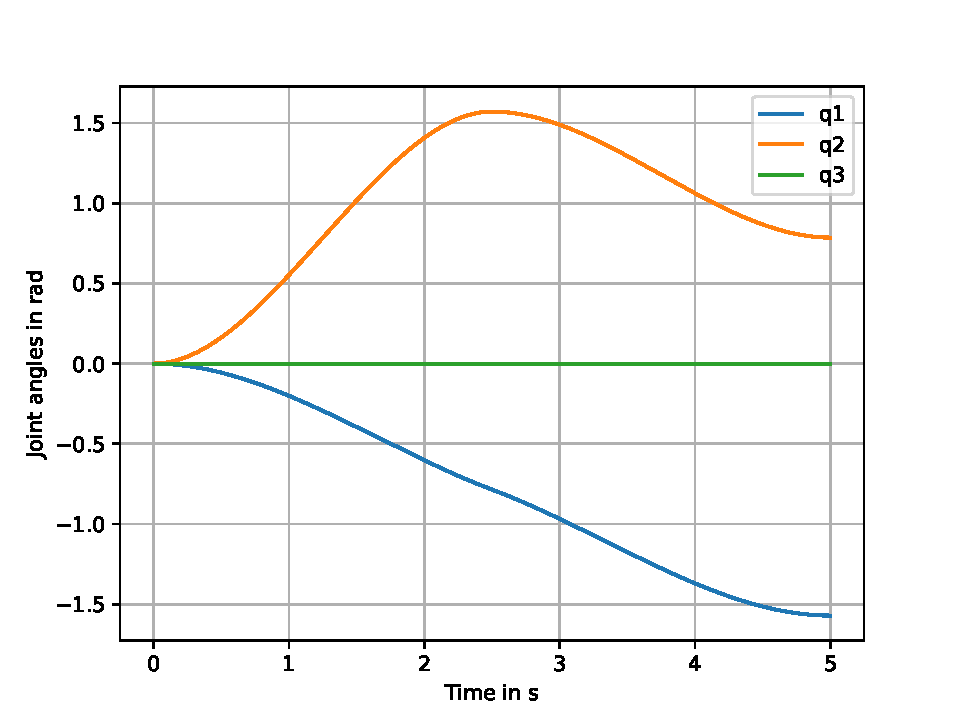
\includegraphics[width=0.8\textwidth]{SRC/Cubic_Spline.pdf}
   \end{center}
  \caption{Cubic Spline trajectory joint angles with respect to time.}
  \label{fig:CubicSplinePlot}
\end{figure}

\subsection{B2 - Trajcetory Generation}
\subsubsection{a}

In this task we need to write a function that calculates the time Tf that it takes for the trajectory from start to the end to reach a defined angle configuration while fulfilling the constrains defined in the task. 

\begin{equation}
    |\dot{q_i}|\leq \dot{q}_{max_i}(\text{gv.qdmax})
\end{equation}

\begin{equation}
    |\ddot{q_i}|\leq \ddot{q}_{max_i}(\text{gv.qddmax})
\end{equation}

As the task demands no as fast as a possible trajectory or a minimal Tf time, it could be solved trivially. 
One could calculate what the maximum constraints are and simply calculate the time Tf by the equation. 

\begin{equation}
    t_f= \frac{|q_{end}-q_{start}|}{\gamma\cdot \dot{q}_{max_i}}
\end{equation}

Where $ 0\leq \gamma \leq 1$ is a factor that we choose arbitrarily low, to definitely fulfill the constraints but not have the fastest trajectory implementation. \newline 
However, it was decided that it was more interesting to try to approach this task from a demand of minimum rise time while still fulfilling constraints sufficiently. For this several calculations had to be made in order to find out how to calculate the minimum Tf depending on the change in angle $q_{end}- q_{start}$ and the velocity/acceleration constraint. For this purpose, the first two equations must be found to fulfill the max velocity and max acceleration criteria and then a rule must be made to choose the stricter criteria. Because if for example, the user sets the max acceleration to a small value and the max velocity to a relatively high value, the Tf should be chosen that way that it fulfills the stricter criteria of acceleration. 

\newline 
In the following the start angle configuration and starting time will be called $q_s$ and $t_s$ respectively and the final configuration time when its reached are called $q_f$ and $t_f$ respectively.
As there is no via in the trajectory generation and the initial velocity should be zero, the equation for the trajectory generation can be simplified to the following.

\begin{equation}
    q(t) = a_{1} + a_{3} \cdot (t-t_{s})^2 + a_{4}\cdot (t-t_{s})^3
    \label{eq:splineOneAdj}
\end{equation}

With the first and second derivatives being Equation \ref{eq:splineDer1} and \ref{eq:splineOneDer2}. 

\begin{equation}
    \dot{q}(t) =  2\cdot a_{3} \cdot (t-t_{s}) + 3 \cdot a_{4}\cdot (t-t_{s})^2
    \label{eq:splineDer1}
\end{equation}

\begin{equation}
    \ddot{q}(t) = 2\cdot a_{3} + 6 \cdot a_{4}\cdot (t-t_{s})
    \label{eq:splineOneDer2}
\end{equation}

As we assume that the starting and end velocity is zero we can plug in the formulas for $a_{i}$ in Equations \ref{eq:splineDer1} and \ref{eq:splineOneDer2}

\begin{equation}
    \dot{q}(t) =  2 \cdot \frac{3(q_{f}-q_{s})}{(t_{f}-t_{s})^2} \cdot (t-t_{s}) + 3 \cdot \frac{-2(q_{f}-q_{s})}{(t_{f}-t_{s})^3}\cdot (t-t_{s})^2
    \label{eq:splineDer1A}
\end{equation}

\begin{equation}
    \ddot{q}(t) = 2\cdot \frac{3(q_{f}-q_{s})}{(t_{f}-t_{s})^2} + 6 \cdot \frac{-2(q_{f}-q_{s})}{(t_{f}-t_{s})^3}\cdot (t-t_{s})
    \label{eq:splineOneDer2A}
\end{equation}

First lets investigate the maximum velocity criteria. The Equation \ref{eq:splineDer1A} is a parabola and from it can be deduced that when the change in angle $q_f$-$q_s$ is positive, it has a maximum and if the change is negative it has only a minimum. As the velocity starts and ends at a value of zero this indicates that the max absolute velocity (positive or negative sign) is reached at the maximum/minimum of the function. 
\newline
The next consequential step is to find the point in time for the maxima and input this time point in the Equation \ref{eq:splineOneAdj} to find out its value at this point in time. 

\begin{equation}
    \ddot{q}(t)= 0=\frac{6(q_{f}-q_{s})}{(t_{f}-t_{s})^2} - \frac{12(q_{f}-q_{s})(t-t_{s})}{(t_{f}-t_{s})^3}
\end{equation}

\begin{equation}
    t_{|\dot{q}_{max}|}=\frac{t_f-t_s}{2}
\end{equation}

Reinsert this into the velocity Equation \ref{eq:splineDer1A} to get the maximum velocity and insert it in the initial velocity constraint.

\begin{equation}
   \dot{q}_{max_i} \geq |\dot{q}(t_{|\dot{q}_{max}|})|
\end{equation}


\begin{equation}
    \dot{q}_{max_i} \geq|\frac{6(q_{f}-q_{s})}{(t_{f}-t_{s})^2} \cdot (\frac{t_f-t_s}{2}-t_{s}) - \frac{6(q_{f}-q_{s})}{(t_{f}-t_{s})^3}\cdot (\frac{t_f-t_s}{2}-t_{s})^2|
    \label{eq:splineDerPutIn}
\end{equation}


\begin{equation}
    \frac{ \dot{q}_{max_i} \cdot (t_{f}-t_{s})^3}{|6(q_{f}-q_{s})|} \geq |    (t_{f}-t_{s}) \cdot (\frac{t_f-t_s}{2}-t_{s}) - (\frac{t_f-t_s}{2}-t_{s})^2|
    \label{eq:splineDePutIn2}
\end{equation}

In our case we can simply define $t_s$ to be zero, as we can program a simple time variable that is set to the current time during the init function of the trajectory generation. This simplifies the formula and provides us with the following equation. 


\begin{equation}
    t_f \geq \frac{|1.5(q_f-q_s)|}{\dot{q}_{max}}
    \label{eq:TFVelocityCriteria}
\end{equation}

This equation shows that for a specific change in angle and a predefined max angular velocity the $t_f$ must be at least equal to the formula to reach the maximum velocity. 
To test the formula assume the case that the maximum absolute allowed angular velocity is $\frac{\pi}{4}\frac{rad}{s}$, $q_s$=0, $q_f=\frac{\pi}{2}$ and $t_s=0$. Inserting this in Equation \ref{eq:TFVelocityCriteria}, provides us with a $t_f=3$. Inserting this in Equation \ref{eq:splineOneAdj} and calculate $a_3$ and $a_4$ accordingly provides us with the trajectory spline polynomial. 



\begin{equation}
    q_{test}(t) =  \frac{3(q_{f}-q_{s})}{t_{f}^2} \cdot t^2 + \frac{-2(q_{f}-q_{s})}{t_{f}^3}\cdot t^3
    \label{eq:SplineTrajExample}
\end{equation}

\begin{equation}
    q_{test}(t) =  \frac{\pi}{6} \cdot t^2 - \frac{\pi}{27}\cdot t^3
    \label{eq:SplineTrajExample}
\end{equation}

\begin{equation}
    \dot{q}_{test}(t) =  \frac{\pi}{3} \cdot t - \frac{\pi}{9}\cdot t^2
    \label{eq:SplineTrajExample}
\end{equation}

\begin{figure}[H]
    \centering
    % Subfigure 1
    \begin{subfigure}[t]{0.48\textwidth}
        \centering
        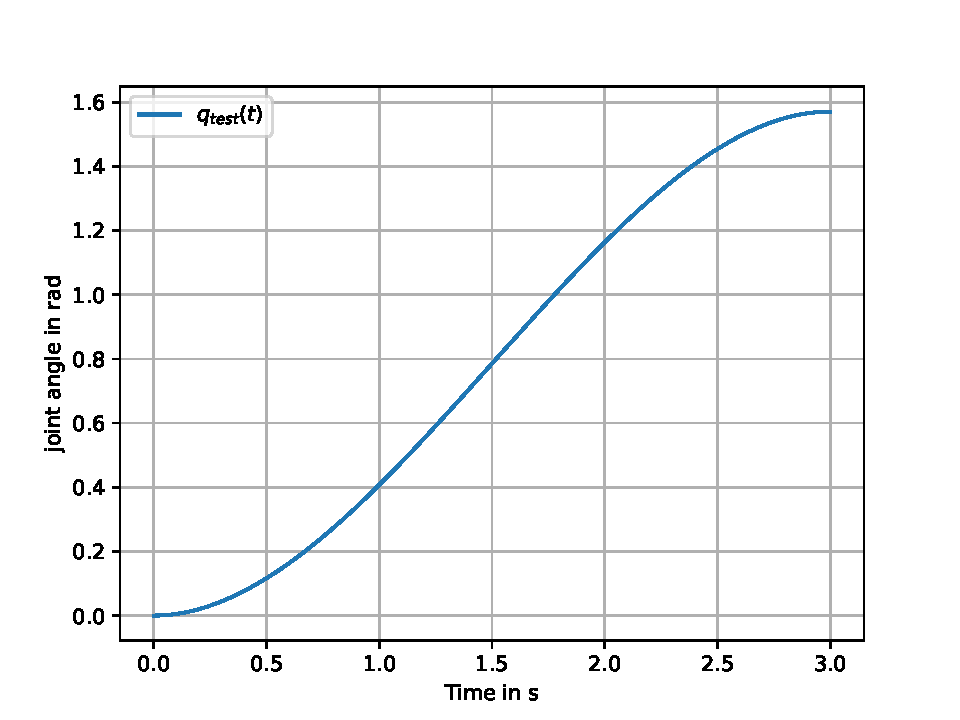
\includegraphics[width=\textwidth]{SRC/SplineExampleAngle.pdf} % Replace with your image
        \caption{ $q_{test}$ plotted over time.}
        \label{fig:subfig1}
    \end{subfigure}
    \hfill
    % Subfigure 2
    \begin{subfigure}[t]{0.48\textwidth}
        \centering
        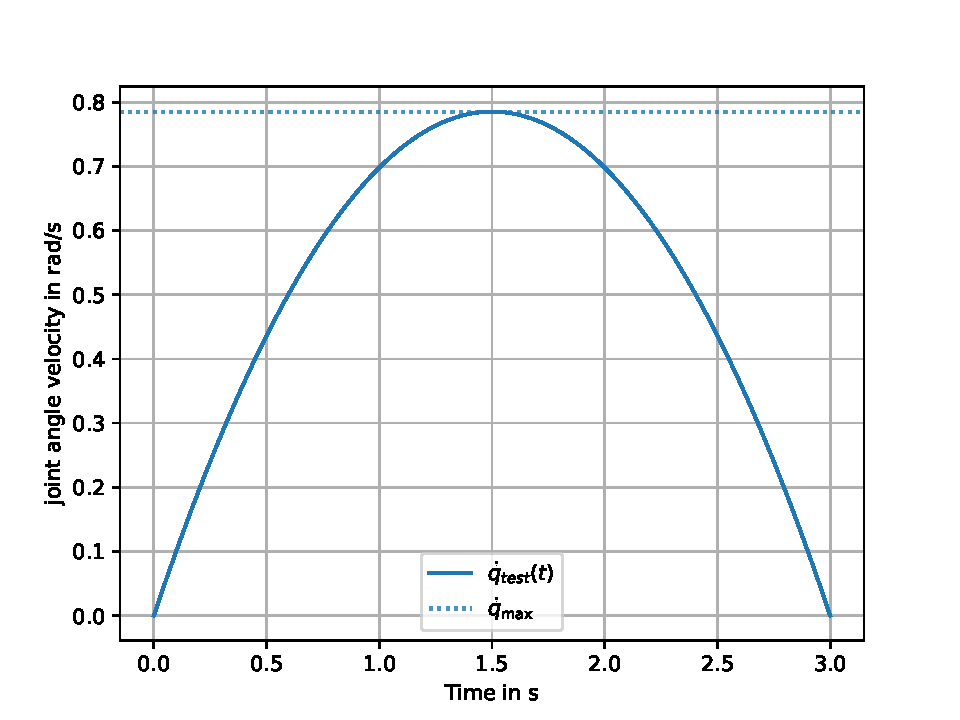
\includegraphics[width=\textwidth]{SRC/SplineExampleVelocity.pdf} % Replace with your image
        \caption{$\dot{q}_{test}$ plotted with specified $\dot{q}_{max}$.}
        \label{fig:subfig2}
    \end{subfigure}
    
    \caption{Cubic spline trajectory of $q_{test}$ and $\dot{q}_{test}$.}
    \label{fig:SplineExample}
\end{figure}


As we can see the derived Equation \ref{eq:TFVelocityCriteria} for the shortest execution time $t_f$ possible with the maximum angular velocity as possible works exactly as intended. However, it might be later beneficial to adjust it by adding a safety margin to the maximum allowed velocity, so that in the real tests we do not overshoot the max velocity. 
\newline

Now that the minimum criteria according to the velocity is clear its time to look at the acceleration. The acceleration of the cubic spline polynomial is a linear term which absolute maximum at timepoint $t_s$ and $t_f$. This seems plausible when looking at Figure \ref{fig:subfig1} as in the beginning and in the end the absolute acceleration is maximum and in the middle, a nearly constant velocity is reached. Therefore we know that $\ddot{q}(t)$ will be max for $t=t_s$. To get the $t_f$ condition to fulfill the $|\ddot{q}(t)| \leq \ddot{q}_{max}$, we need to insert the timepoint $t=t_s$ in Equation \ref{eq:splineOneDer2A} and assume that we can choose $t_s$ to be our starting timepoint so that $t_s=0$ holds.

\begin{equation}
    \ddot{q}_{max} \geq  |\ddot{q}(t)|
\end{equation}

\begin{equation}
    \ddot{q}_{max} \geq |\frac{6(q_{f}-q_{s})}{t_{f}^2}|
    \label{eq:splineOneDerAtMax}
\end{equation}

\begin{equation}
    t_f \geq \sqrt{\frac{|6(q_{f}-q_{s})|}{\ddot{q}_{max}}}
    \label{eq:SplineAccCriteria}
\end{equation}

Assuming the same example as previous but we say that the maximum allowed acceleration $\ddot{q}_{max}=\frac{\pi}{3}\frac{rad}{s}$. According to the Equation \ref{eq:SplineAccCriteria} the compute minimum $t_f$= would also be 3s. So we generate the same polynomial spline as previously but plot it alongside the maximum allowed acceleration.

\begin{figure} [H]
   \begin{center}
        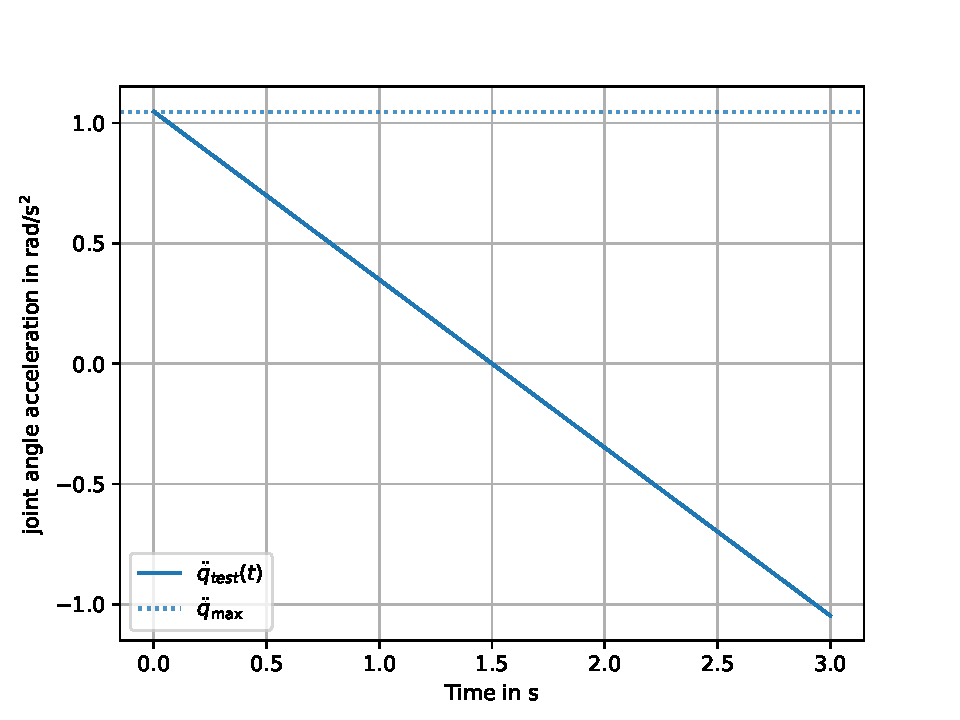
\includegraphics[width=0.5\textwidth]{SRC/SplineExampleAcceleration.pdf}
   \end{center}
  \caption{Cubic spline trajectory of $\ddot{q}_{test}$ and $\ddot{q}_{max}$.}
  \label{fig:AcceSpline}
\end{figure}

Figure \ref{fig:AcceSpline} shows us that the formula for the minimum $t_f$ with acceleration contains is working perfectly. To select the stricter of the two criteria so that $t_f$ fulfills both constraints, the Equation can be written as follows.

\begin{equation}
    t_f=max(\ \frac{|1.5(q_f-q_s)|}{\dot{q}_{max}}, \sqrt{\frac{|6(q_{f}-q_{s})|}{\ddot{q}_{max}}}\ ) 
\end{equation}
\newpage
However, it is important to add that all the joint angles have to reach their desired trajectory at the same time, so the $t_f$ must be chosen according to the largest $q_i - q_{d_i}$ (current joint angle - desired joint angle). Therefore the final formula which computes the common minimum $t_f$ for all joint trajectories which fulfills both constraints while still being as fast as possible can be defined as.

\begin{equation}
    t_{f1}=max(\ \frac{|1.5(q_{f1}-q_{s1})|}{\dot{q}_{max}}, \sqrt{\frac{|6(q_{f1}-q_{s1})|}{\ddot{q}_{max}}}\ ) 
\end{equation}

\begin{equation}
    t_{f2}=max(\ \frac{|1.5(q_{f2}-q_{s2})|}{\dot{q}_{max}}, \sqrt{\frac{|6(q_{f2}-q_{s2})|}{\ddot{q}_{max}}}\ )
\end{equation}

\begin{equation}
    t_{f3}=max(\ \frac{|1.5(q_{f3}-q_{s3})|}{\dot{q}_{max}}, \sqrt{\frac{|6(q_{f3}-q_{s3})|}{\ddot{q}_{max}}}\ )
    \label{eq:q3tfmin}
\end{equation}

\begin{equation}
    t_f_{min}=max(t_{f1},t_{f2},t_{f3})
\end{equation}


In the code we added an additional safety margin to the calculated $t_f_{min}$, by in creasing it by 5\% of its length.

\subsubsection{c) Trajectory to a specific point}

\begin{figure} [H]
   \begin{center}
        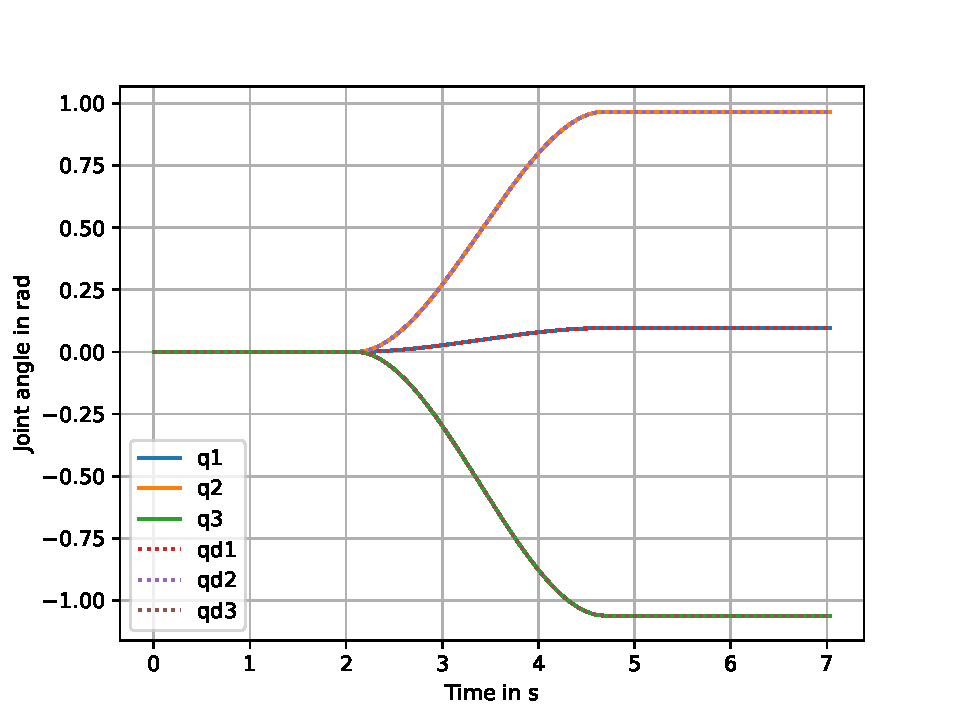
\includegraphics[width=0.7\textwidth]{SRC/Puma_spline_q_qd.pdf}
   \end{center}
  \caption{q and qd of the cubic spline trajectory of proj1 with gains $k_{p1}$=54400, $k_{p2}$=44400, $k_{p3}$=10400, $k_{v1}$=240, $k_{v2}$=140, $k_{v3}$=140.}
  \label{fig:PumaCubicSplineQ}
\end{figure}


\begin{figure} [H]
   \begin{center}
        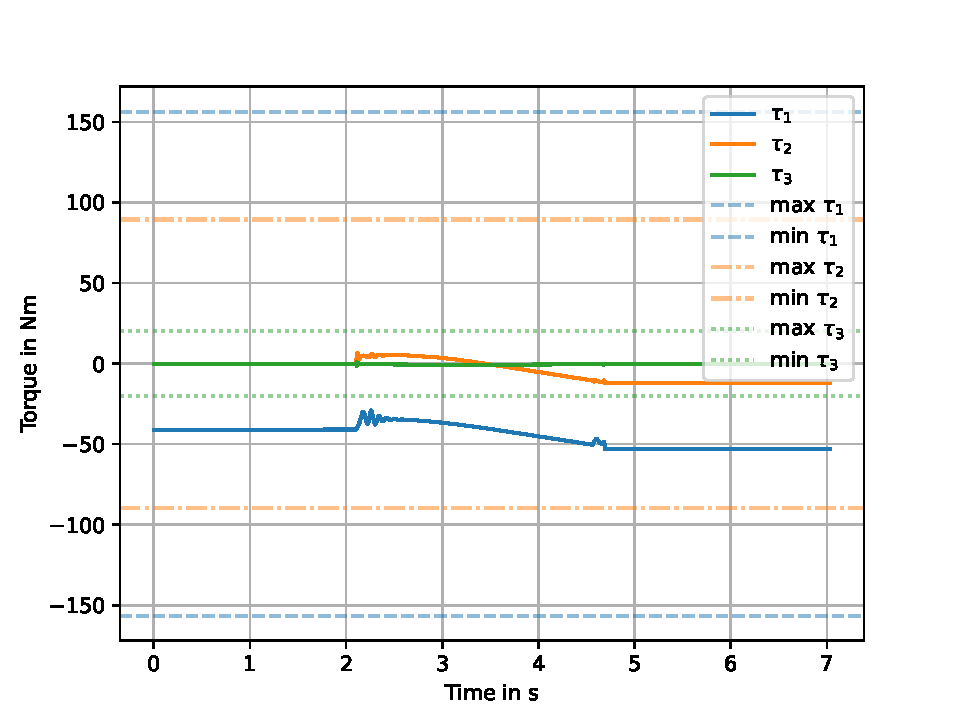
\includegraphics[width=0.7\textwidth]{SRC/Puma_spline_tau.pdf}
   \end{center}
  \caption{Torque of the cubic spline trajectory of proj1 with gains $k_{p1}$=54400, $k_{p2}$=44400, $k_{p3}$=10400, $k_{v1}$=240, $k_{v2}$=140, $k_{v3}$=140.}
  \label{fig:PumaCubicSplineTau}
\end{figure}

As one can see in Figures \ref{fig:PumaCubicSplineQ} and \ref{fig:PumaCubicSplineTau} the cubic spline trajectory is well followed by proj1 control. The gains can be chosen significantly higher than in the assignment 1 as the differences in angle change only very slowly with the trajectory per timestep. As one can see this also shows itself in the relatively small torque that is needed to initiate the motion. 
\newline

In the following Figure \ref{fig:PumaCubicSplineDQDQQ} the angular velocity and acceleration is shown. From the figures we can presume that the stricter constraint was the max acceleration as the acceleration plot of $q_3$ is closest to the max allowed value.
From the GUI of the Pumasim we can extract that the maximum allowed velocity is per default set to 45$\frac{\circ}{s}$ and max acceleration to 60$\frac{\circ}{s^2}$. When writing those in $rad/s$ and $rad/s^2$ we can insert it in Equation \ref{eq:q3tfmin} as $q_3$ has the largest change in angle and will therefore require the longest $t_f$. 

\begin{equation}
    t_{f_{min}}
    =max(\ \frac{|1.5\cdot(-1.061\ rad)|}{\frac{\pi}{4}\frac{rad}{s}}, \sqrt{\frac{|6\cdot(-1.061\ rad)|}{\frac{\pi}{3}\frac{rad}{s^2}}}\ ) \approx max(2.03s, 2.47s) =  2.47s
\end{equation}

Additionally the previously mentioned 5\% safety margin were added by the code to the execution time of the spline so that $t_f$=$ t_{f_{min}}\cdot 1.05\approx$ 2.59s. This execution time is shown in the Figures and especially in Figure \ref{fig:PumaCubicSplineDDQ} one can see that the acceleration of $q_3$ is close to the max acceleration with a margin of around 5\%.

\begin{figure}[H]
    \centering
    % Subfigure 1
    \begin{subfigure}[t]{0.48\textwidth}
        \centering
        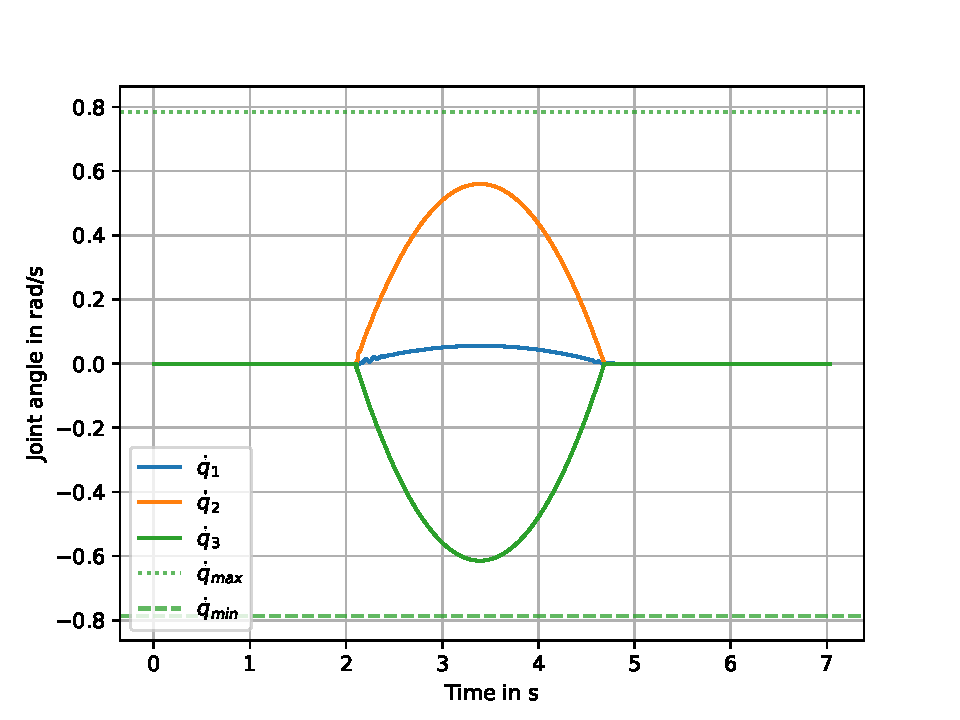
\includegraphics[width=\textwidth]{SRC/Puma_spline_dq.pdf} % Replace with your image
        \caption{ $\dot{q}$ plotted with specified $\dot{q}_{max}$.}
        \label{fig:PumaCubicSplineDQ}
    \end{subfigure}
    \hfill
    % Subfigure 2
    \begin{subfigure}[t]{0.48\textwidth}
        \centering
        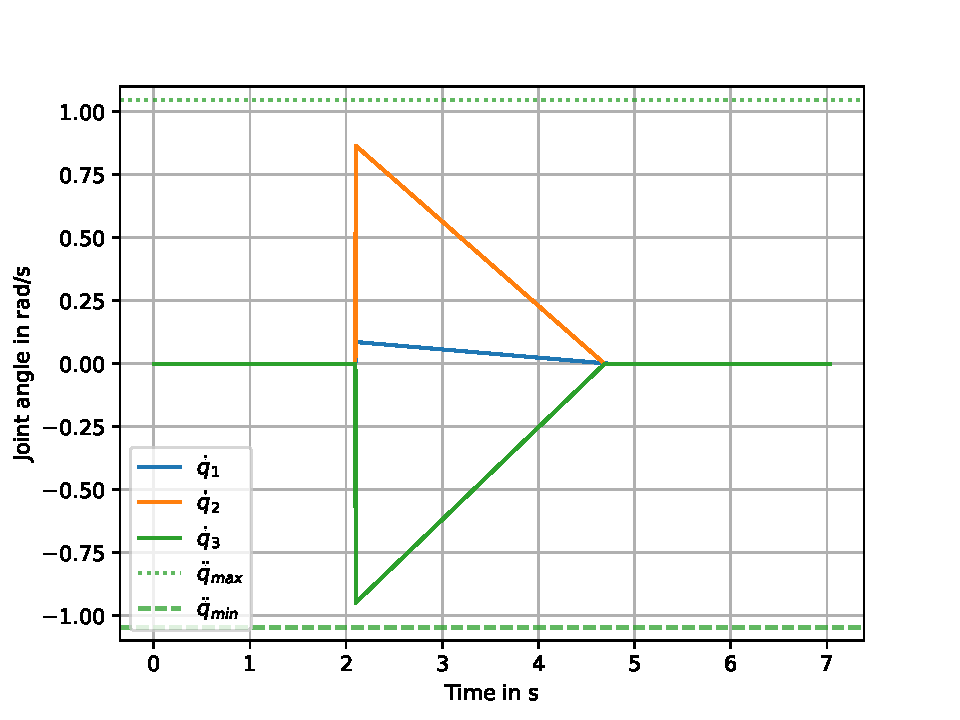
\includegraphics[width=\textwidth]{SRC/Puma_spline_ddq.pdf} % Replace with your image
        \caption{$\ddot{q}$ plotted with specified $\ddot{q}_{max}$.}
        \label{fig:PumaCubicSplineDDQ}
    \end{subfigure}
    
    \caption{$\dot{q}$ and $\ddot{q}$ of the cubic spline trajectory of proj1 with gains $k_{p1}$=54400, $k_{p2}$=44400, $k_{p3}$=10400, $k_{v1}$=240, $k_{v2}$=140, $k_{v3}$=140.$ and $\dot{q}_{test}$.}
    \label{fig:PumaCubicSplineDQDQQ}
\end{figure}